\begin{frame}
\frametitle{When the model is wrong about the topology}
\large
\begin{centering}

\textcolor{DarkBlue}{\only<1>{One bottleneck}\only<2>{Two bottlenecks}}

\end{centering}
\vspace{\baselineskip}
\vspace{\baselineskip}

\only<1>{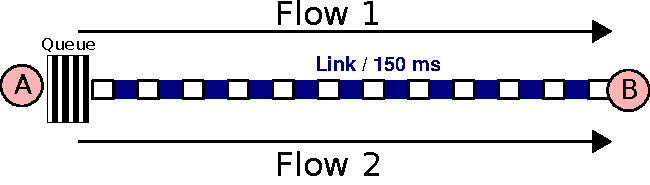
\includegraphics[width=\textwidth]{onelink.pdf}}\only<2>{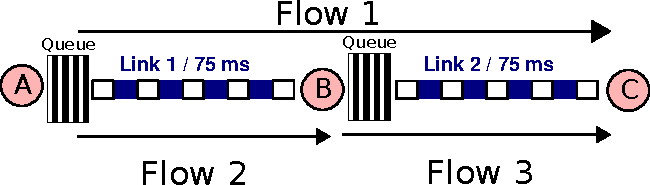
\includegraphics[width=\textwidth]{twolink.pdf}}

\end{frame}

\begin{frame}
\frametitle{When the model is wrong about the topology}
\begin{centering}

\noindent \only<1>{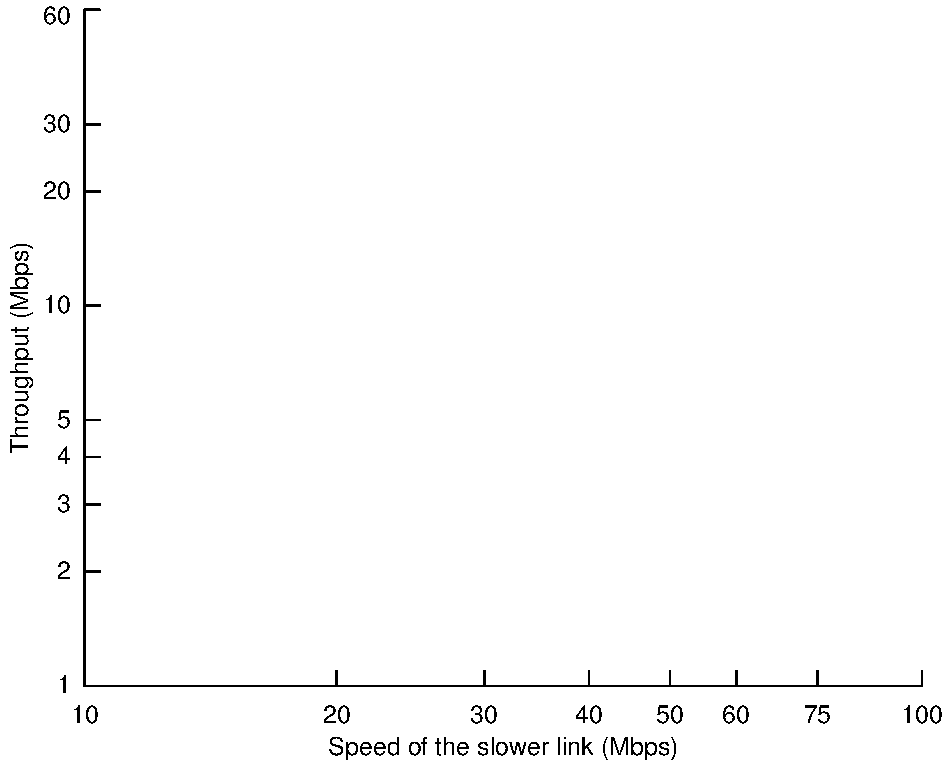
\includegraphics[width=3.4 in]{multilink-background.pdf}}\only<2>{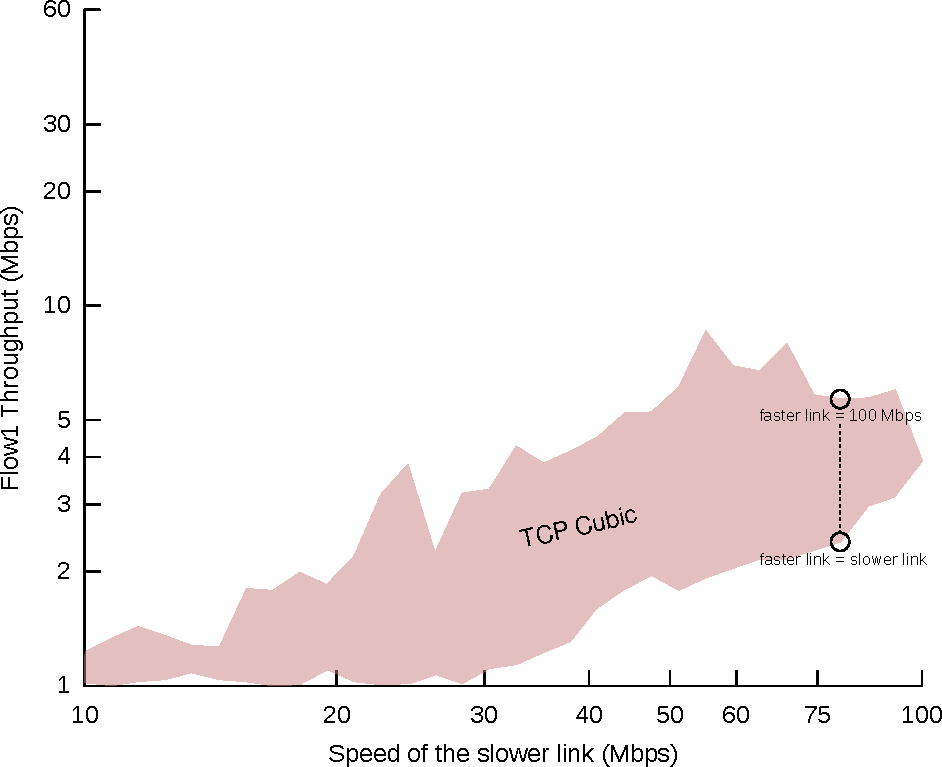
\includegraphics[width=3.4 in]{multilink-cubic.pdf}}\only<3>{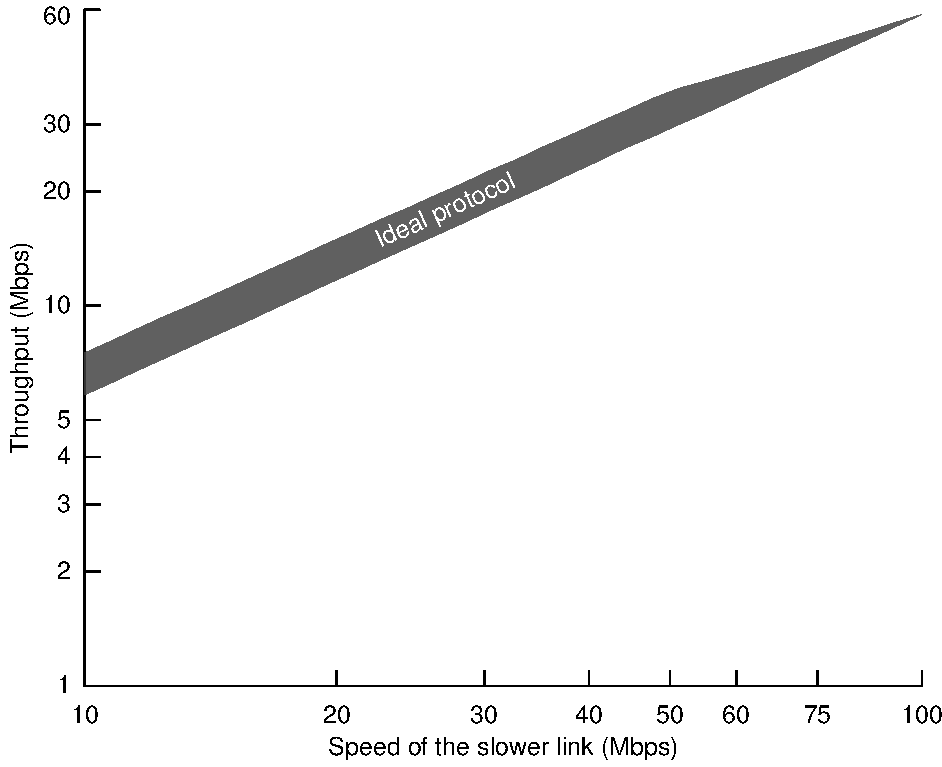
\includegraphics[width=3.4 in]{multilink-omniscient.pdf}}\only<4>{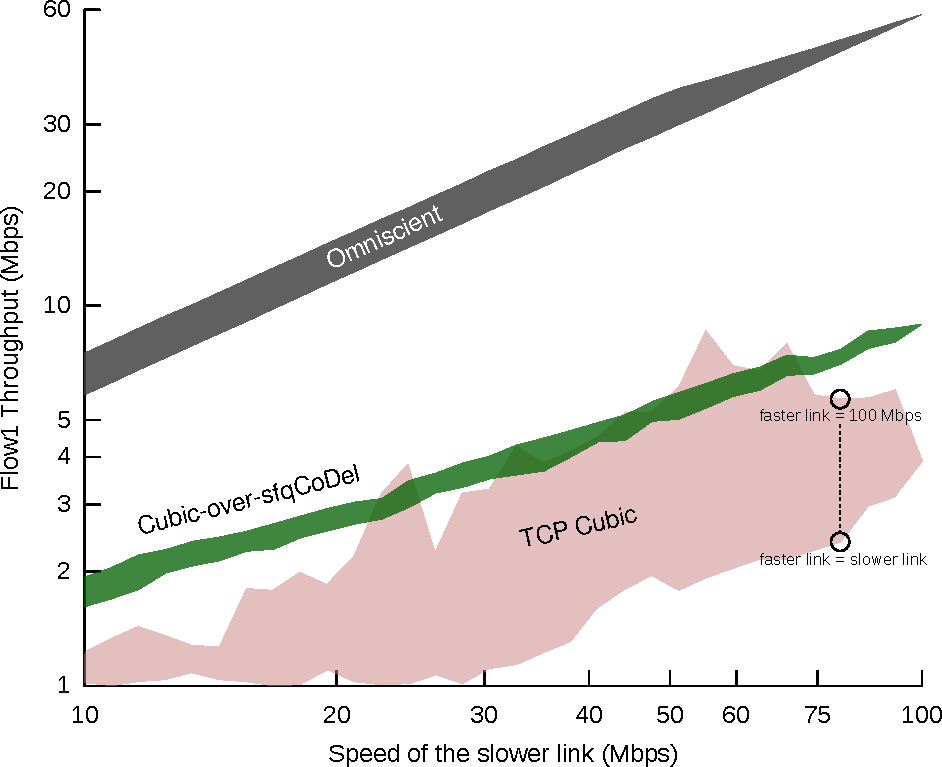
\includegraphics[width=3.4 in]{multilink-codel.pdf}}\only<5>{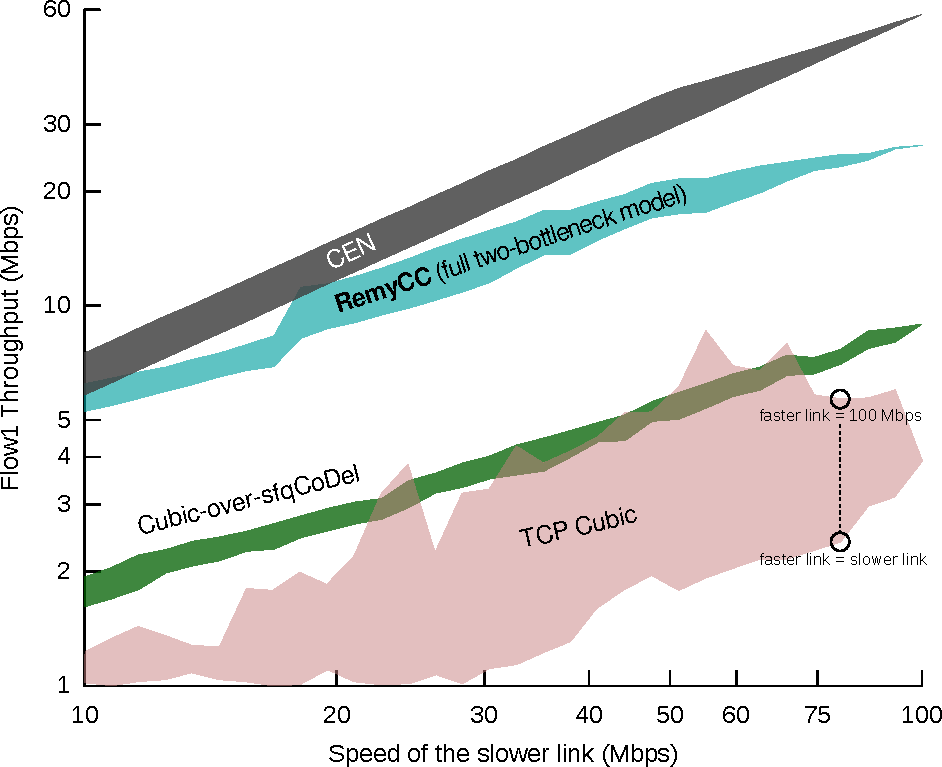
\includegraphics[width=3.4 in]{multilink-twolink.pdf}}\only<6>{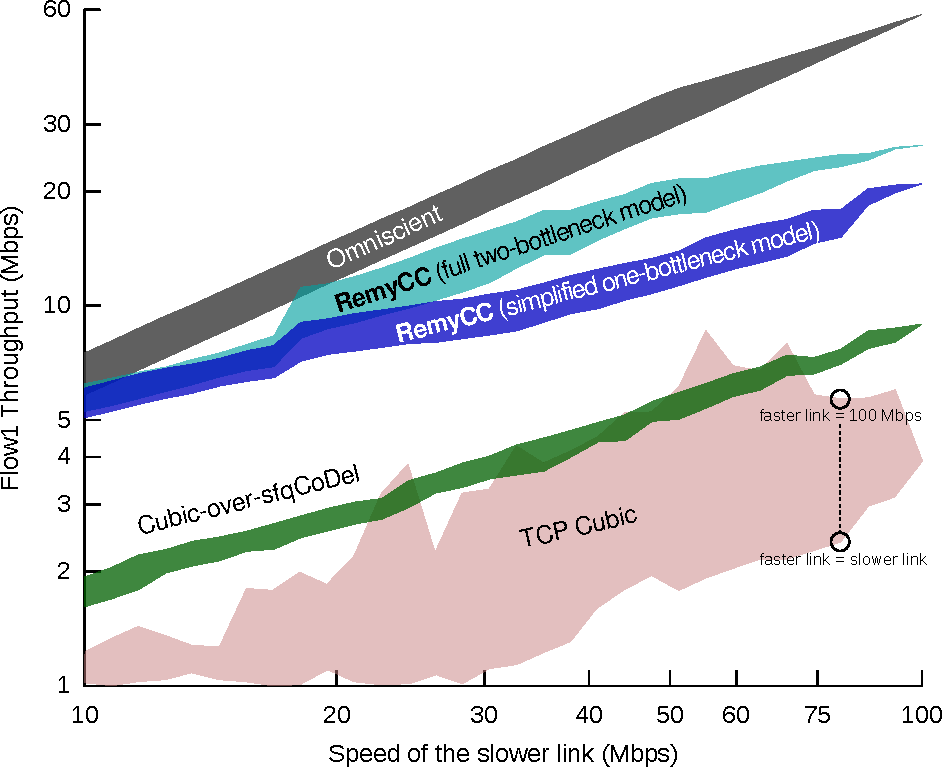
\includegraphics[width=3.4 in]{multilink-onelink.pdf}}

\end{centering}
\end{frame}

\begin{frame}
\frametitle{When the model is wrong about the topology}
\begin{centering}

Simplifying a two-link network to a single-link network only modestly hurts performance

\end{centering}
\end{frame}
